\subsubsection{Projection of Run-2 ATLAS searches for MSSM heavy Higgs bosons}
%-------------------------------------------------------------------------------
\paragraph{Introduction}
\label{sec:intro}
%-------------------------------------------------------------------------------

The discovery of a Standard Model (SM) like Higgs boson ~\cite{ATLASHiggsJuly2012, CMSHiggsJuly2012}
at the Large Hadron Collider (LHC)~\cite{LHC} has provided important insight into the mechanism of
electroweak symmetry breaking. However, it remains possible that the discovered particle is part
of an extended scalar sector, a scenario that is favored by a number of theoretical arguments~\cite{Djouadi:2005gj,Branco:2011iw}.
Searching for additional Higgs bosons is among the main goals of
the High-Luminosity LHC (HL-LHC) programme~\cite{ecfa15}. The Minimal Supersymmetric Standard
Model (MSSM)~\cite{Djouadi:2005gj,Fayet:1976et,Fayet:1977yc} is one of the well motivated extensions
of the SM\@. Besides the SM-like Higgs boson, the MSSM requires two additional neutral Higgs bosons:
one CP-odd ($A$) and one CP-even ($H$), which in the following are generically called $\phi$.
At tree level, the MSSM Higgs sector depends on only two non-SM parameters, which can be chosen
to be the mass of the CP-odd Higgs boson, $m_A$, and the ratio of the vacuum expectation values
of the two Higgs doublets, $\tan\beta$. Beyond tree level, a number of additional parameters
affect the Higgs sector, the choice of which defines various MSSM benchmark scenarios, such as \mhmodp and hMSSM.
The couplings of the additional MSSM Higgs bosons to down-type fermions are enhanced with respect to
the SM Higgs boson for large $\tan\beta$ values, resulting in increased branching fractions to
$\tau$-leptons and $b$-quarks, as well as a higher cross section for Higgs boson production
in association with $b$-quarks.

The projections presented in this note are extrapolations of the recent results obtained by ATLAS using
the $36.1~\ifb$ \RunTwo dataset~\cite{ATLASRun2Ditau}.  The MSSM Higgs boson with masses of
0.2--2.25\TeV and $\tan\beta$ of 1--58 is searched for in the \lephad and \hadhad decay modes,
where \taulep represents the leptonic decay of a $\tau$-lepton, whereas \tauhad represents the hadronic decay.
The main production modes are gluon--gluon fusion and in association with $b$-quarks.
To exploit the different production modes, events containing at least one $b$-tagged jet enter the $b$-tag
category, while events containing no $b$-tagged jets enter the $b$-veto category. The total transverse
mass ($\mTtot$), as defined in Ref.~\cite{ATLASRun2Ditau}, is used as the final discriminant between
the signal and the background.

In making these extrapolations, the assumption is made that the planned upgrades to the ATLAS detector and
improvements to reconstruction algorithms will mitigate the effects of the higher pileup which can reach up
to 200 in-time pileup interactions, leading to the overall reconstruction performance matching that of the current detector.
Furthermore, the assumption is made that the analysis will be unchanged in terms of selection and
statistical analysis technique, though the current analysis has not been re-optimised for the HL-LHC datasets.

\paragraph{Extrapolation method}
\label{sec:extrapolation method}
To account for the integrated luminosity increase at HL-LHC, signal and background distributions are scaled by
a factor of $3000/36.1$. Furthermore, to account for the increase in collision energy from $13~\TeV$
to $14~\TeV$, the background distributions are further scaled by a factor 1.18 which assumes the same
parton-luminosity increase for quarks as that for gluons. The cross section of signals in various scenarios
at $14~\TeV$ are given in Ref.~\cite{deFlorian:2016spz}. Possible effects on the kinematics and the $\mTtot$
shape due to the collision energy increase are neglected for this study. The scaled $\mTtot$ distributions
for the four signal categories and one for the top control region are shown in
Figures~\ref{fig:mTtotDistributionsSR} and~\ref{fig:mTtotDistributionsCR}. These distributions are used in
the statistical analysis.

\begin{figure}[!ht]
    \centering
        \subfloat[\lephad $b$-veto category]{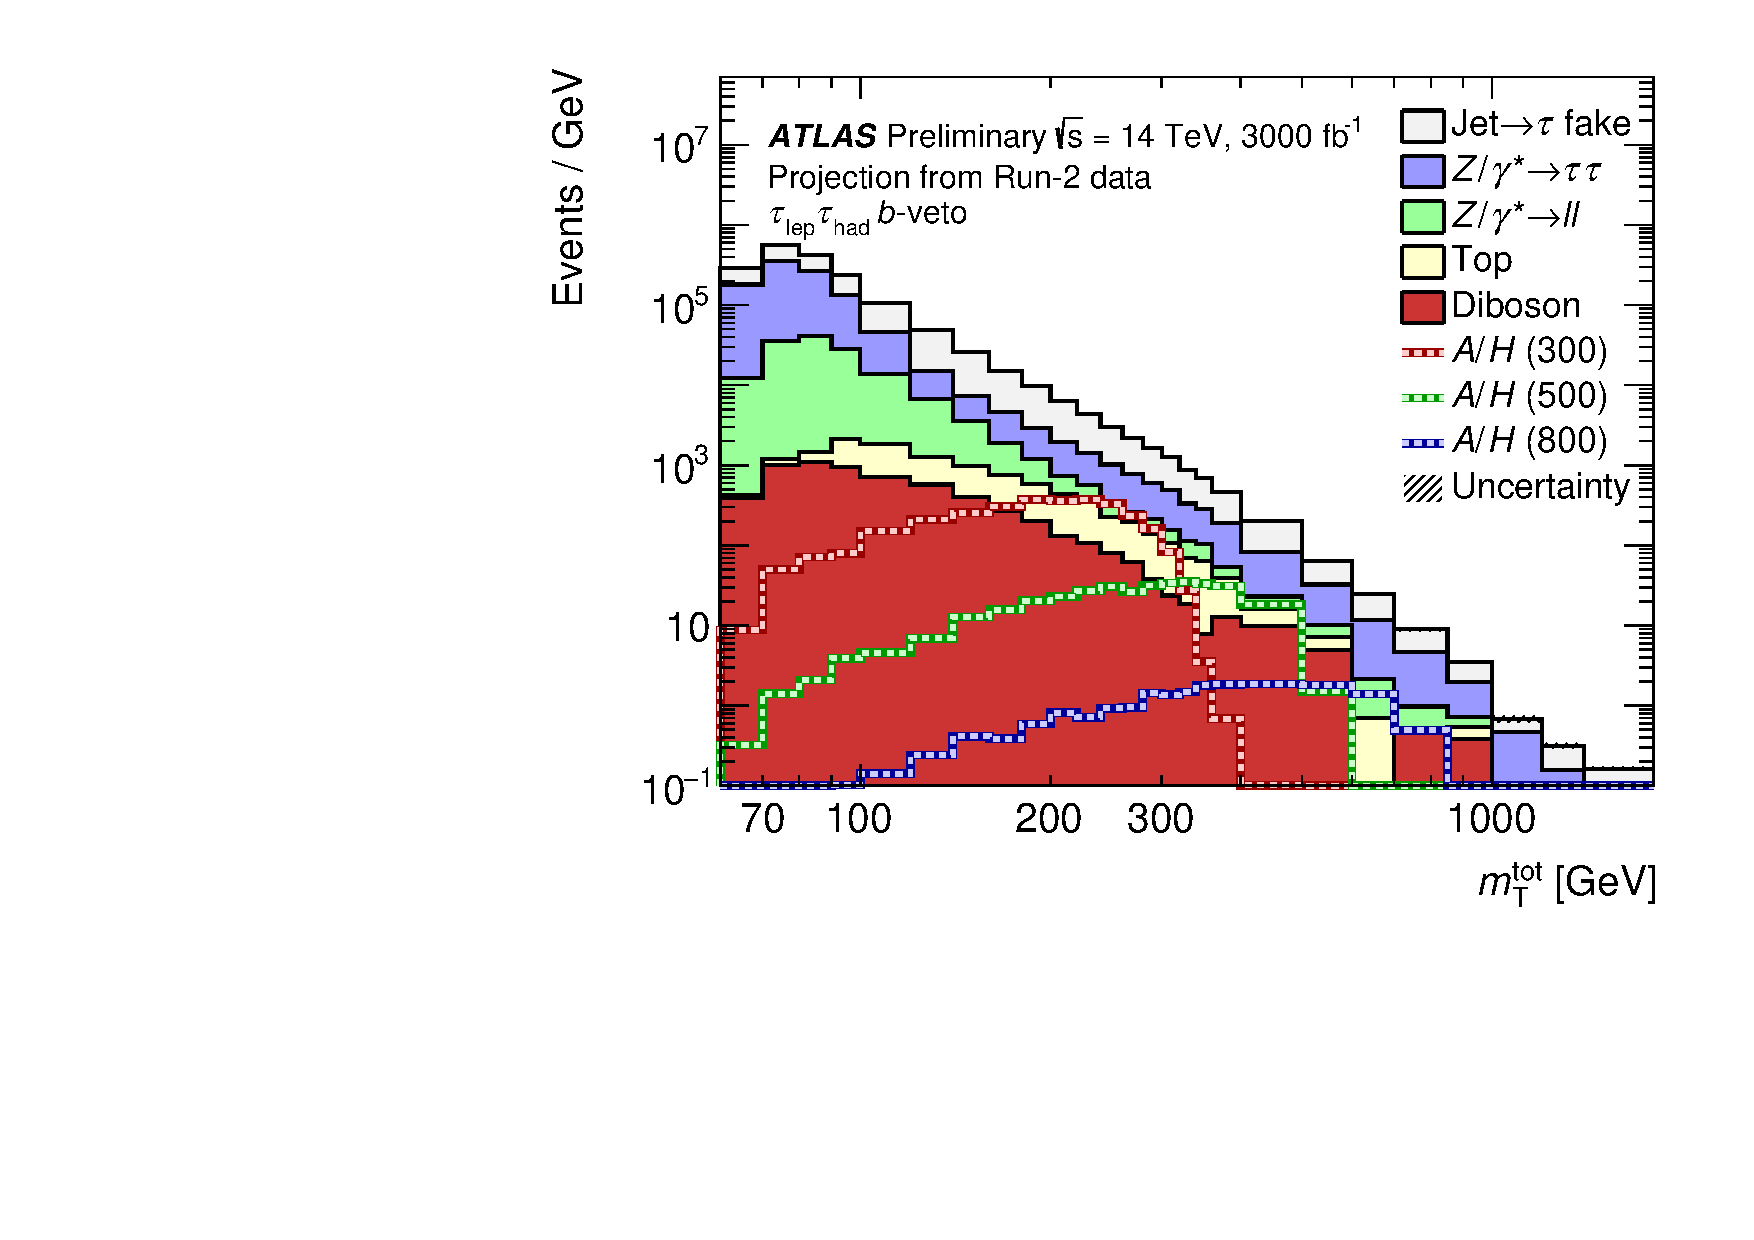
\includegraphics[width=0.45\columnwidth]{\main/section9/plots/c170_postfit_lephad_bveto_MTtot__highlumi.pdf}}
        \qquad
        \subfloat[\lephad $b$-tag category]{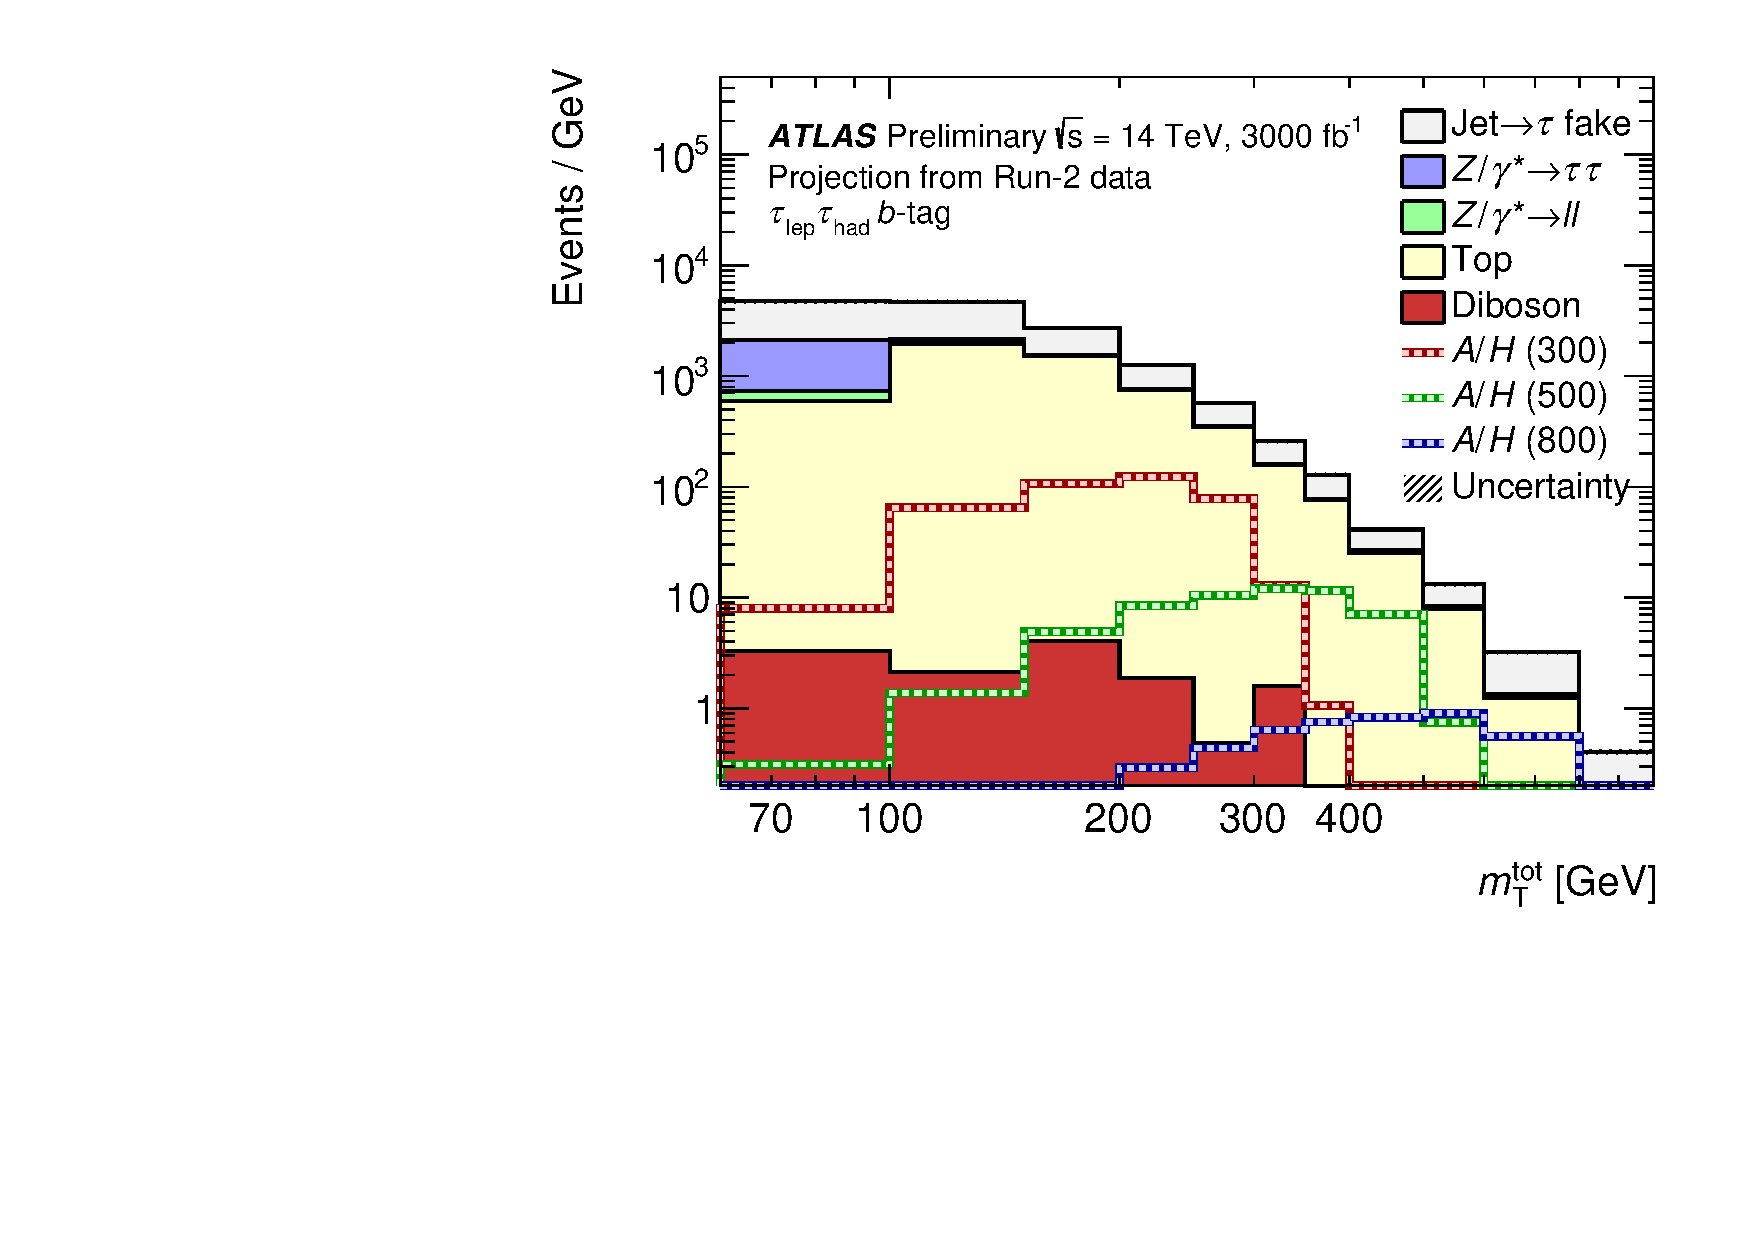
\includegraphics[width=0.45\columnwidth]{\main/section9/plots/c171_postfit_lephad_btag_MTtot__highlumi.pdf}}
        \qquad
        \subfloat[\hadhad $b$-veto category]{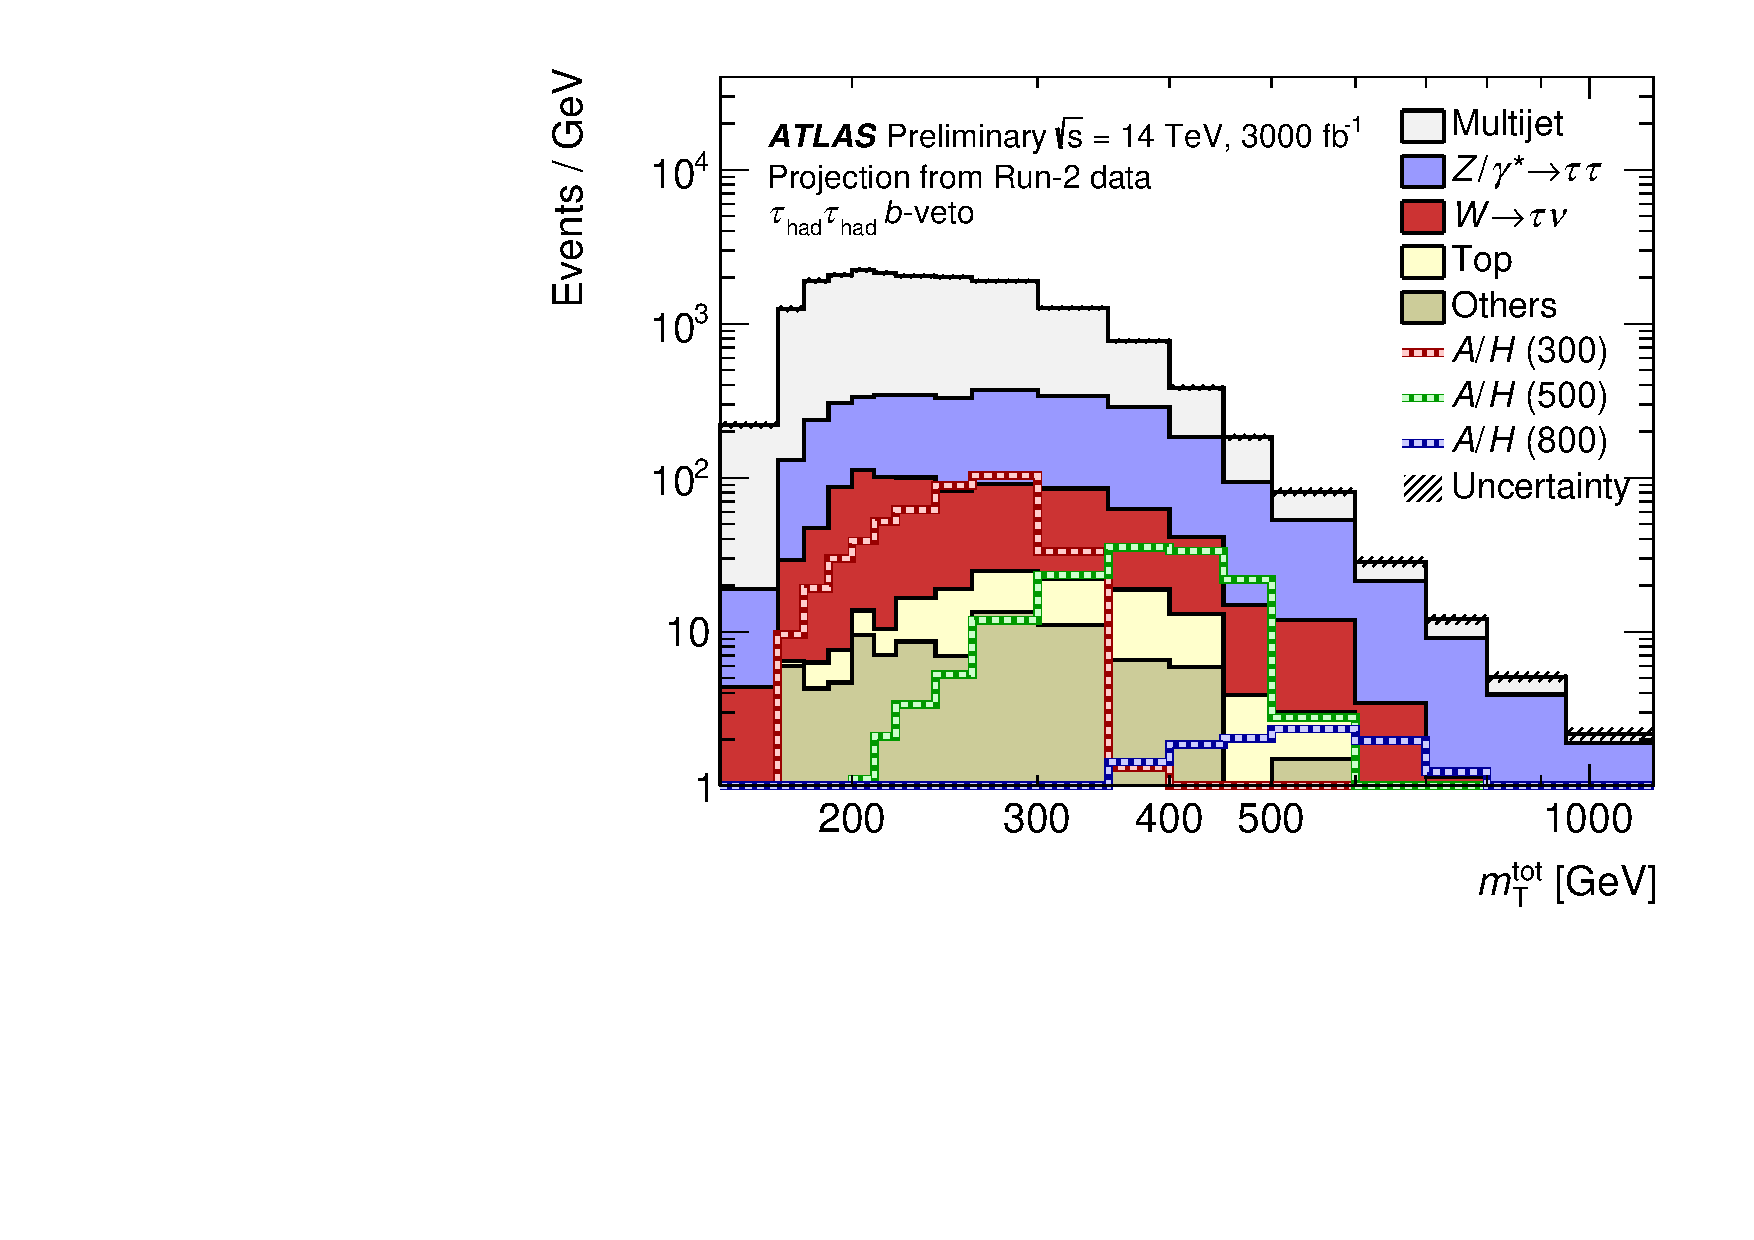
\includegraphics[width=0.45\columnwidth]{\main/section9/plots/c20_postfit_hadhad_bveto_MTtot__highlumi.pdf}}
        \qquad
        \subfloat[\hadhad $b$-tag category]{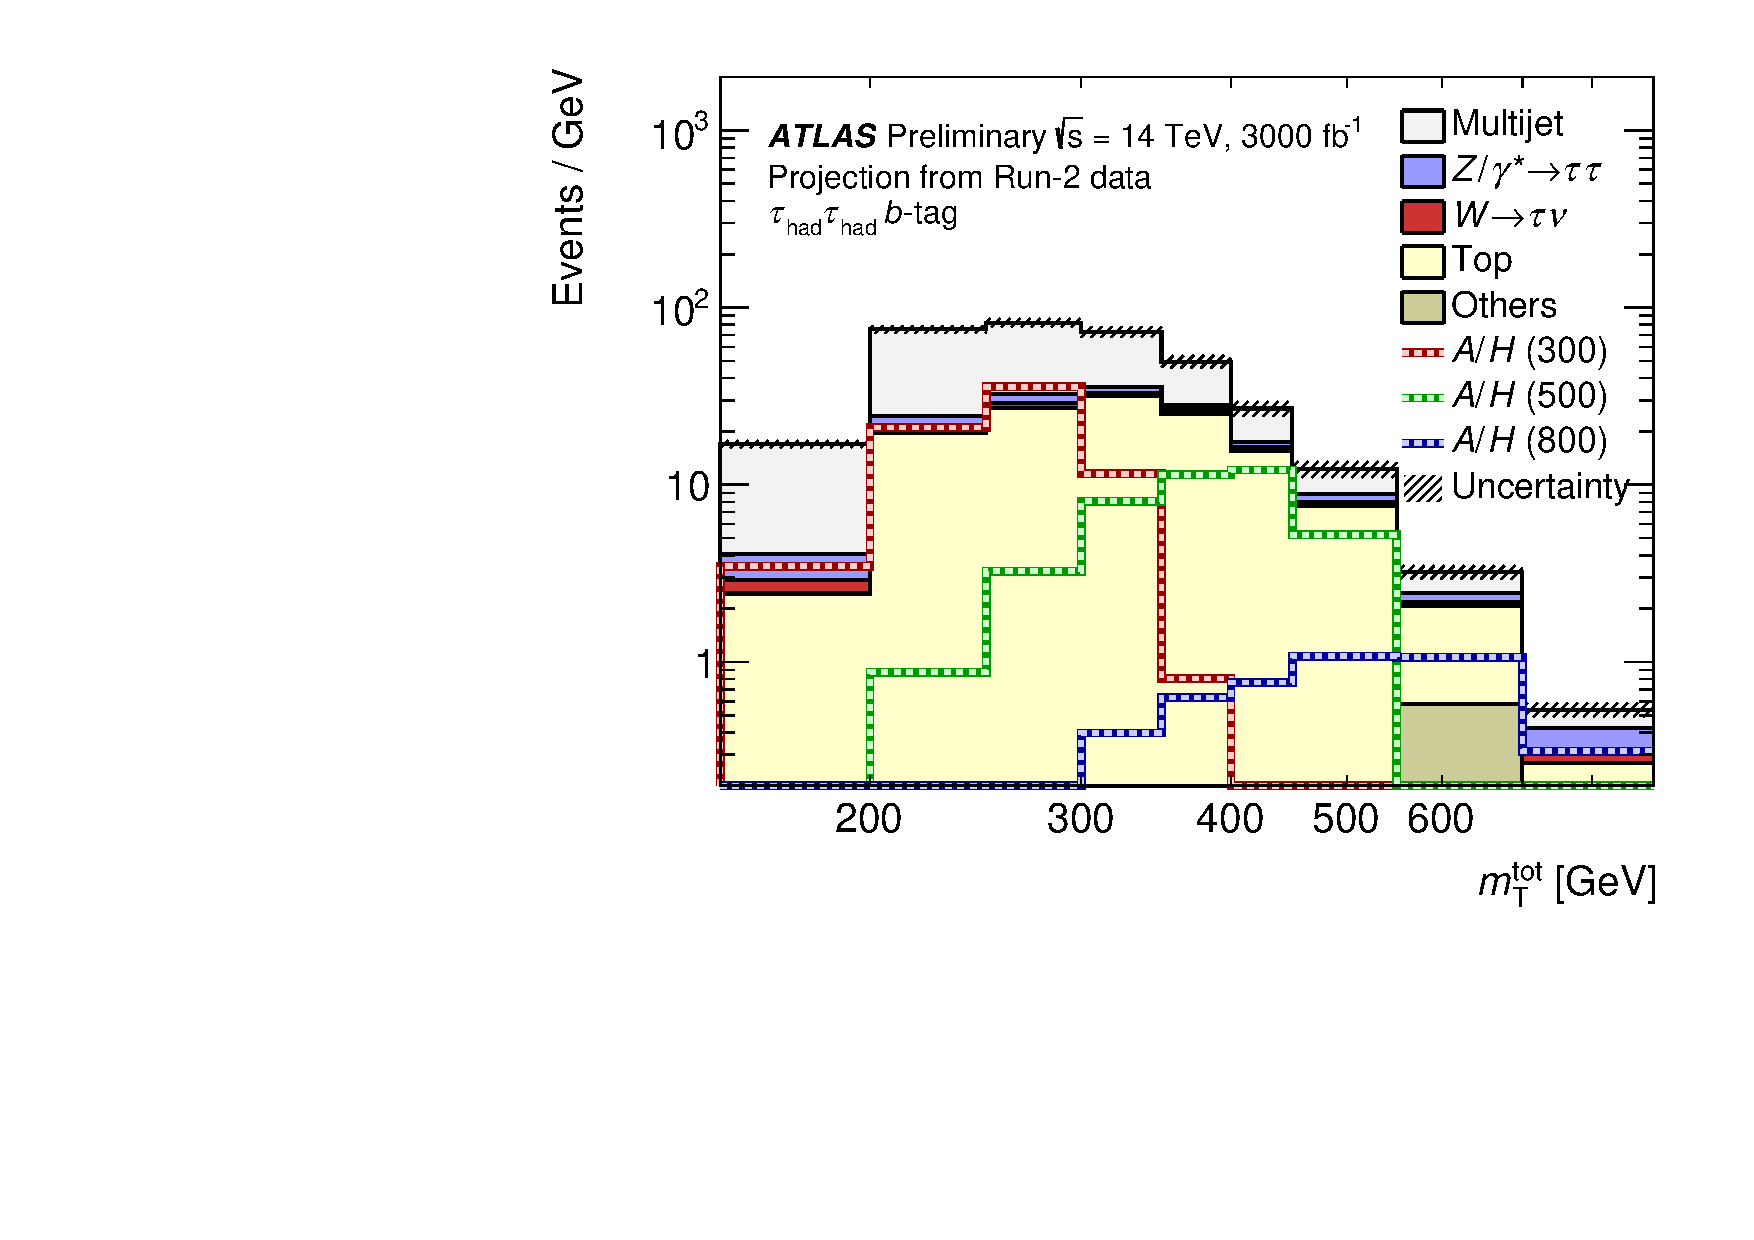
\includegraphics[width=0.45\columnwidth]{\main/section9/plots/c21_postfit_hadhad_btag_MTtot__highlumi.pdf}}
        \caption{Distributions of $\mTtot$ for each signal category. The predictions and uncertainties (including both statistical and systematic components) for the background processes are obtained from the fit under the hypothesis of no signal. The combined prediction for $A$ and $H$ bosons with masses of 300, 500 and 800 \si{\GeV} and $\tan\beta= 10$ in the hMSSM scenario are superimposed. }

    \label{fig:mTtotDistributionsSR}
\end{figure}

\begin{figure}[!ht]
    \centering
        \qquad
        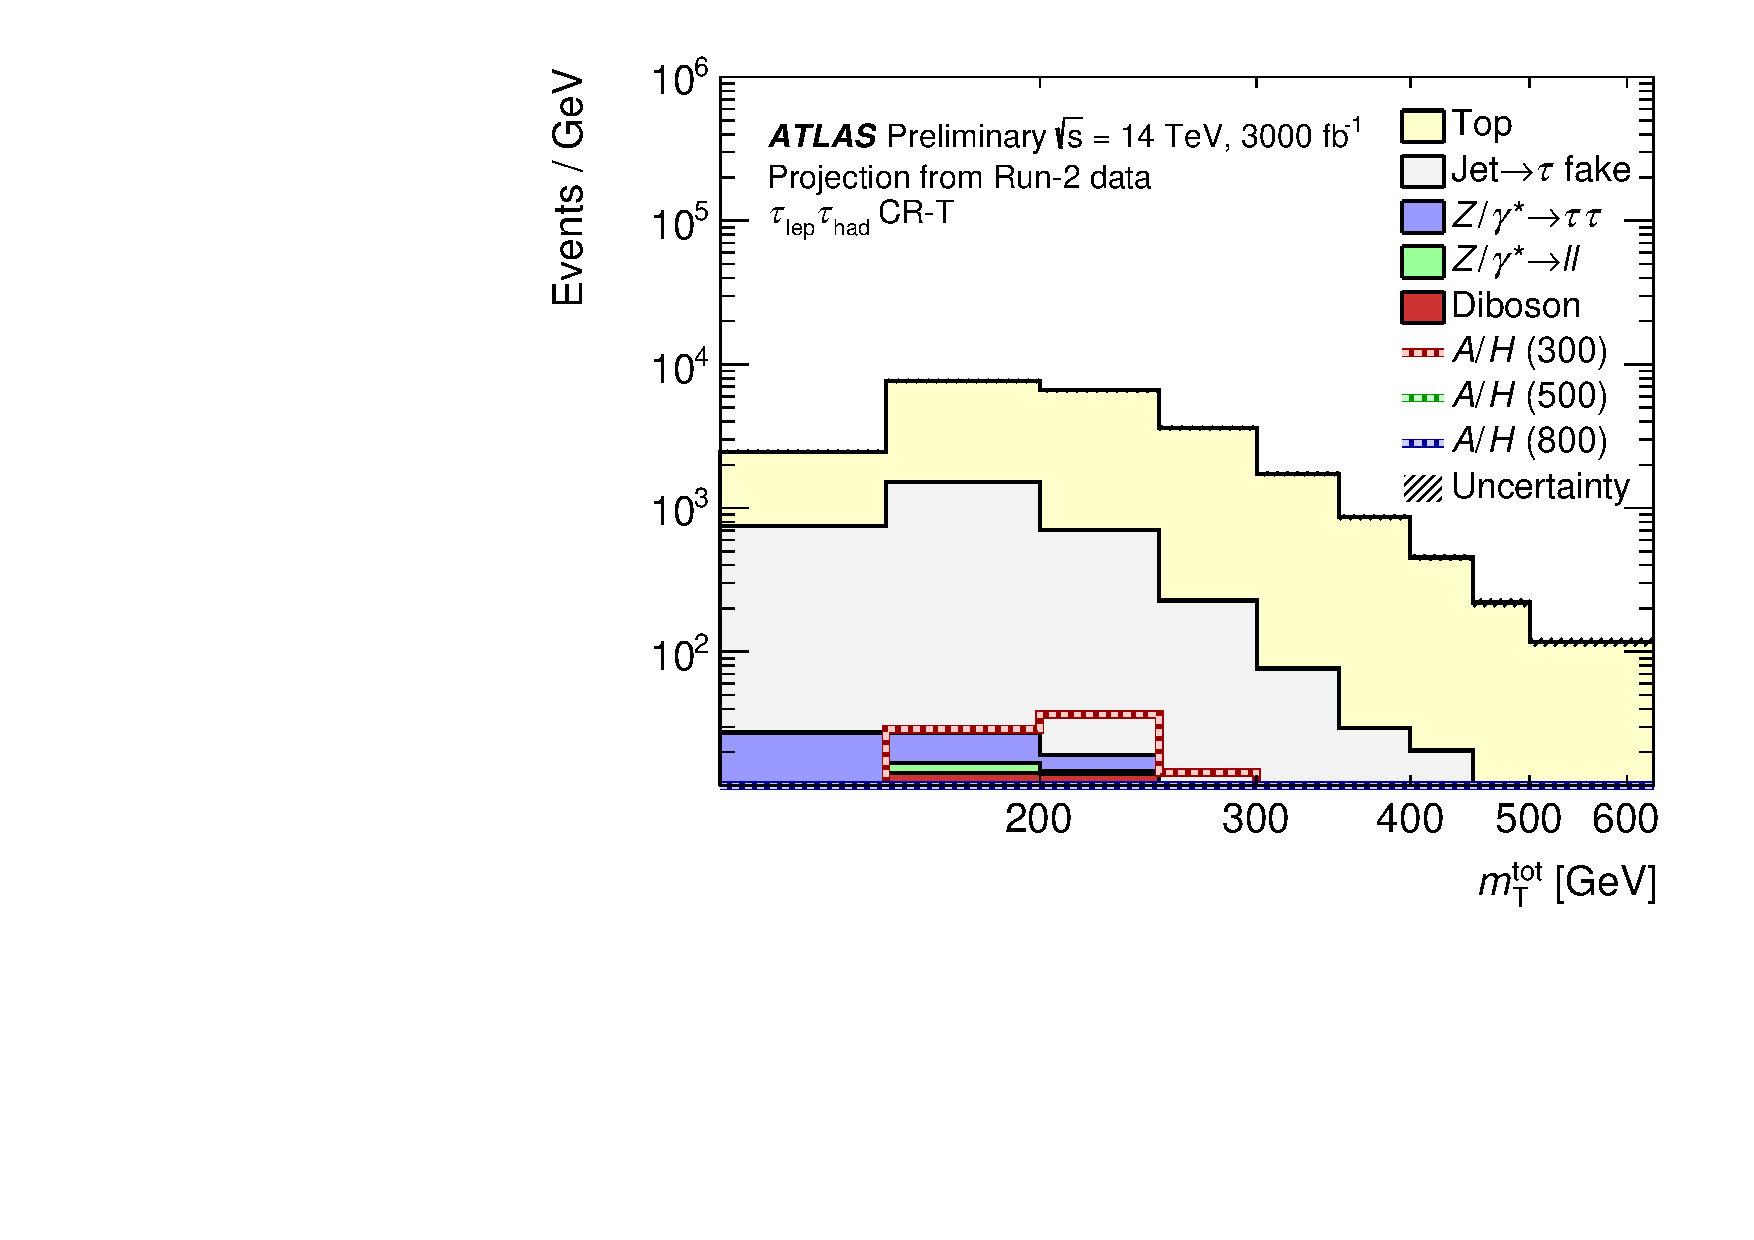
\includegraphics[width=0.5\columnwidth]{\main/section9/plots/c181_postfit_lephad_tcr_MTtot__highlumi.pdf}
        \caption{Distribution of $\mTtot$ distributions in in the top quark enriched control region of the \lephad channel.}
    \label{fig:mTtotDistributionsCR}
\end{figure}

The larger dataset at HL-LHC will give the opportunity to reduce the systematic uncertainties.
The ``Baseline'' scenario for the systematic uncertainty reduction compared to current Run 2 values follows
the recommendation of Ref.~\cite{LHATLASdetectorSystScale}, according to which the systematic uncertainties
associated with $b$-tagging, $\tauhad$ (hadronic $\tau$ decay) and theoretical uncertainties
due to the missing higher order,
the PDF uncertainty, etc., are reduced. The systematic uncertainties associated with the reconstruction
and identification of the high-$\pt$ $\tauhad$ is reduced by a factor of 2 and becomes the leading systematic
uncertainty for a heavy Higgs boson with mass $m_{\phi} > 1~\TeV$. The systematic uncertainty associated
with the modeling of the jet to $\tauhad$ fake background is assumed to be the same as in the current analysis.
For the jet to $\tauhad$ fake background from multijet in \hadhad channel, the modeling uncertainty is mainly
due to the limited data size in the control region and is reduced by a factor of 2. The statistical uncertainties
on the predicted signal and background distributions, defined as the ``template stat.\@ uncertainty'', is determined
by the size of the MC samples and of the data sample in the control region where the \tauhad~ fake factor is applied.
The impact of the template stat.\@ uncertainty is negligible in the Run 2 analysis. Assuming large enough MC
samples will be generated for HL-LHC and sufficient data will be collected at HL-LHC, the uncertainties due to
the sample size is ignored in this extrapolation study.
To quantify the importance of the reduction of systematic uncertainties compared to current Run 2 values,
results (labeled as ``Unreduced'') will also be given with current Run 2 values
except for ignoring the template stat.\@ uncertainty.

%-------------------------------------------------------------------------------
\paragraph{Results}
\label{sec:result}
The $\mTtot$ distributions from the \lephad(separately in the electron and muon channels) and \hadhad signal regions, as well as the top control region, are used in the final combined fit to extract the signal. The statistical framework used to produce the \RunTwo results is documented in Ref.~\cite{ATLASRun2Ditau} and is adapted for this HL-LHC projection study. The results are given in terms of exclusion limits~\cite{CLs_2002}, as well as the 5 $\sigma$ discovery reach for gluon--gluon fusion and $b$-quarks association production modes.

\paragraph{Impact of systematic uncertainties}
The impact of systematic uncertainties on the upper limit of the cross section times branching ratio ($\sigma\times BR(\phi\to\tau\tau)$) in Baseline scenario are calculated by comparing the expected 95\% CL upper limit in case of no systematic uncertainties, $\mu^{95}_{\text{stat}}$, with a limit calculated by introducing a group of systematic uncertainties, $\mu^{95}_i$, as described in Ref.~\cite{ATLASRun2Ditau}. The systematic uncertainty impacts are shown in Figure~\ref{fig:sysimpact, ggH} for gluon--gluon fusion production and Figure~\ref{fig:sysimpact, bbH} for $b$-quarks association production as a function of the scalar boson mass. The major uncertainties are grouped according to their origin, while minor ones are collected as ``Others'' as detailed in Ref.~\cite{ATLASRun2Ditau}.

The impact of systematic uncertainties is significant, as they degrade the expected limits by about 10--150 percent. In the low mass range, the leading uncertainties arise from the estimation of the dominant jet to $\tauhad$ fake background. At high masses, the leading uncertainty is from the reconstruction and identification of high-$\pt$ $\tauhad$. Because $\mu^{95}_{\text{stat}}$ is mainly determined by the data statistical uncertainty. In Figure~\ref{fig:sysimpact, ggH} the impact of the $\tauhad$ related systematic uncertainties decreases after $1~\TeV$ is due to the fact that the results at the higher mass regime are more limited by the data statistical uncertainty, while in Figure~\ref{fig:sysimpact, bbH} the data statistical uncertainty in the \btag category dominates in the high mass regime which leads the high-$\pt$ $\tauhad$ systematic uncertainty less outstanding.

\begin{figure}[!ht]
    \centering
        \subfloat[gluon--gluon fusion production\label{fig:sysimpact, ggH}]{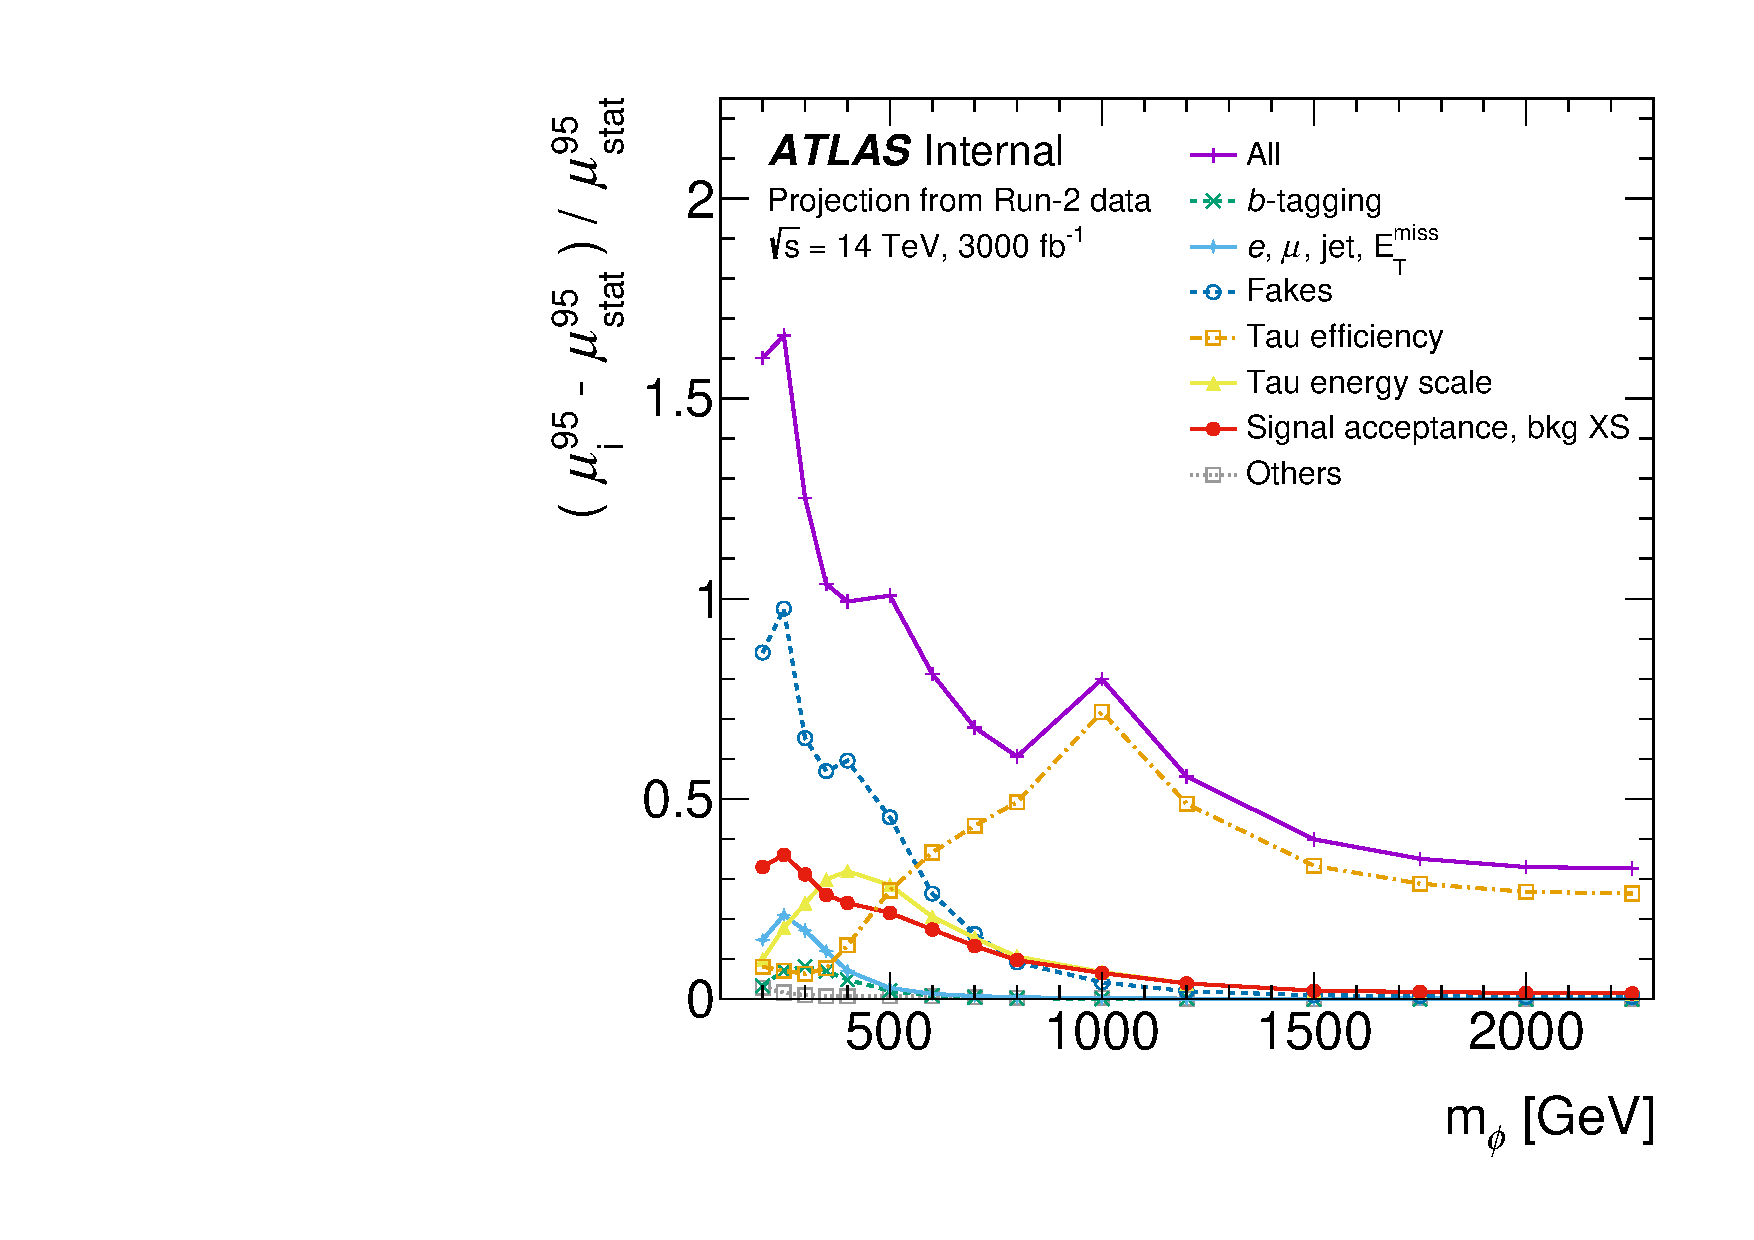
\includegraphics[width=0.4\columnwidth]{\main/section9/plots/ggH__syst_impacts.pdf}}
        \qquad
        \subfloat[$b$-associated production\label{fig:sysimpact, bbH}]{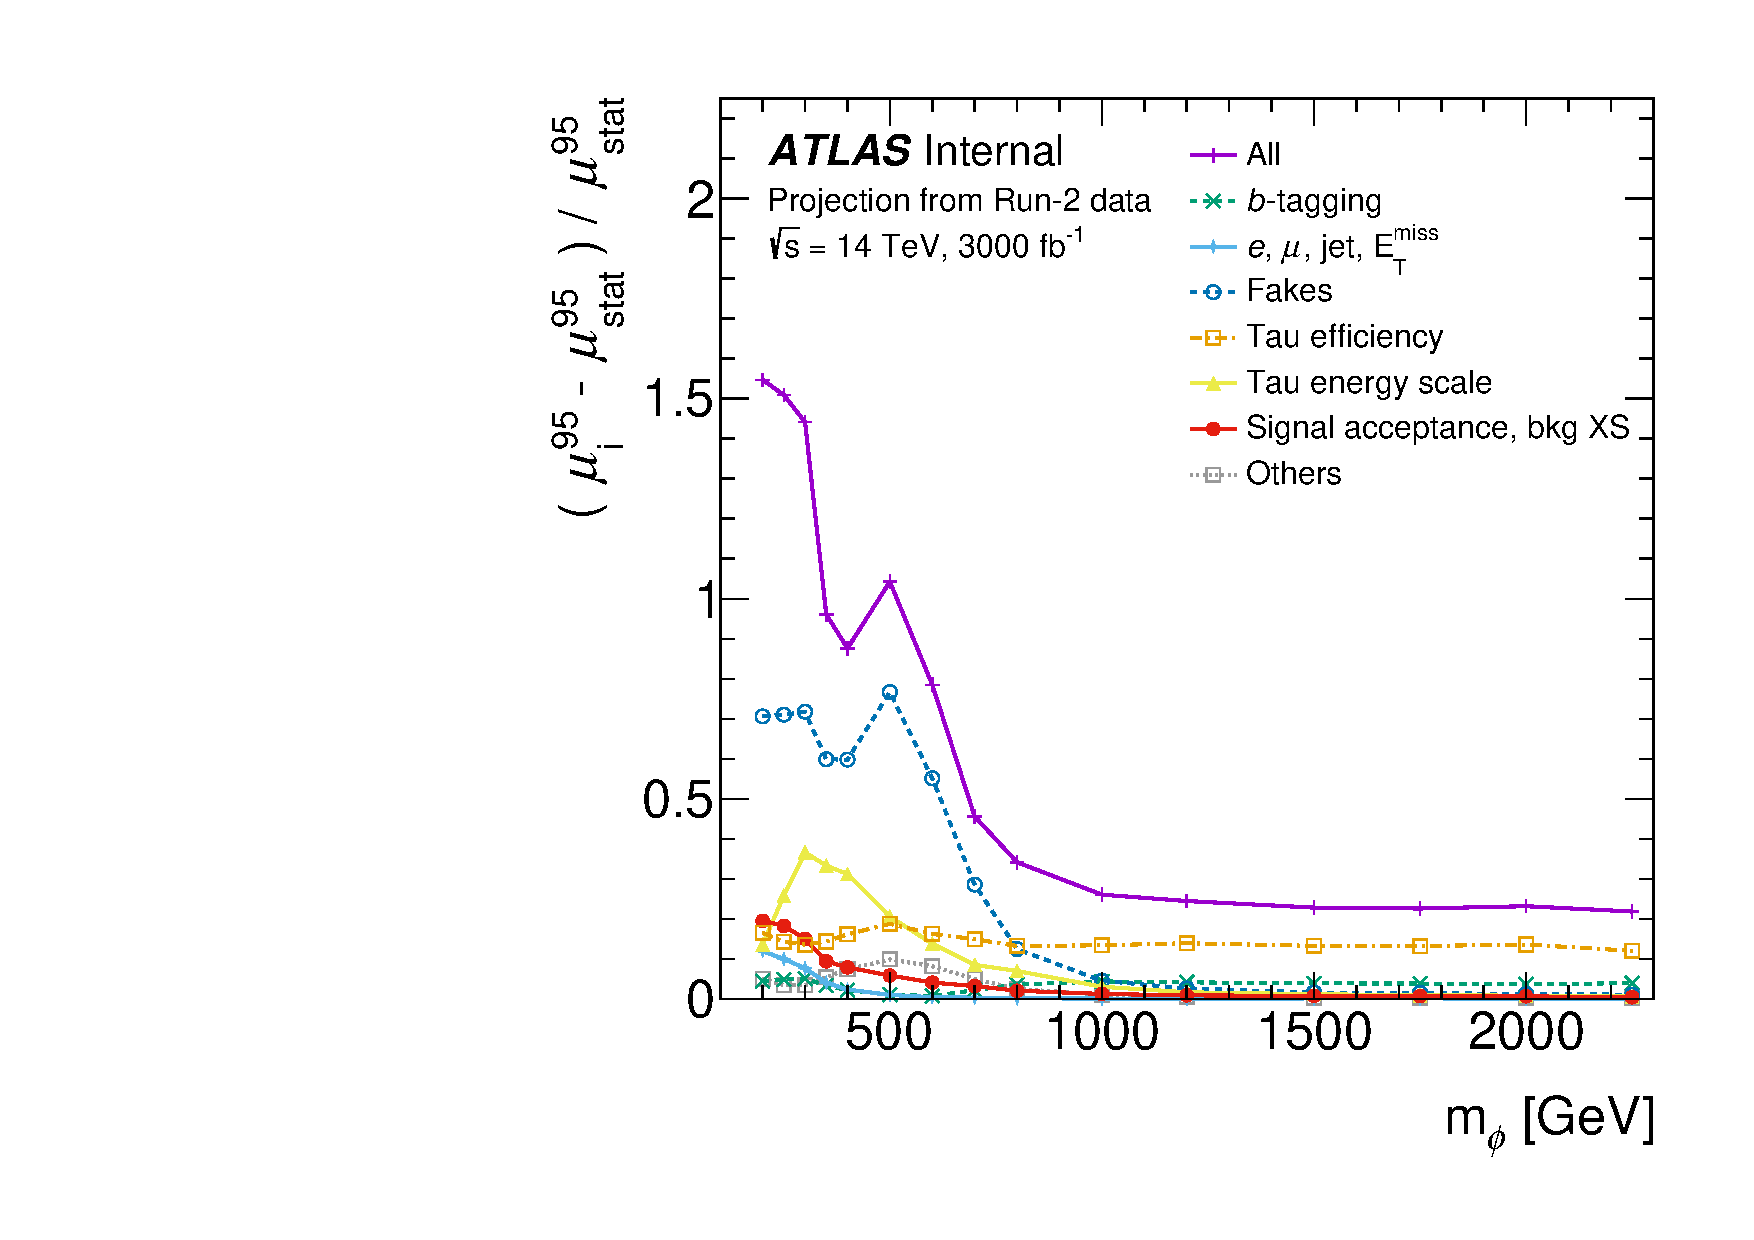
\includegraphics[width=0.4\columnwidth]{\main/section9/plots/bbH__syst_impacts.pdf}}
        \caption{Impact of major groups of systematic uncertainties (Baseline) on the $\phi\to\tau\tau$ 95\% CL cross section upper limits as a function of the scalar boson mass, separately for the (a) gluon--gluon fusion and (b) $b$-associated production mechanisms.}
    \label{fig:sysimpact}
\end{figure}

\paragraph{Cross section limits and discovery reach}
Figure \ref{fig:modelInde} shows the upper limits on the gluon--gluon fusion and $b$-quark associated production cross section times the branching fraction for $\phi\rightarrow\tau\tau$. To demonstrate the impact of systematic uncertainties, the expected exclusion limits with different systematic uncertainty scenarios are shown, as well as the Run 2 expected results~\cite{ATLASRun2Ditau}. The peaking structure around $m_\phi = 1~\TeV$ in figure \ref{fig:modelInde, ggH} is due to the impact of the high-$\pt$ $\tauhad$ systematic uncertainty. The 5 $\sigma$ sensitivity line in the same figure illustrates the smallest values of the cross section times the branching fraction for which discovery level can be reached at HL-LHC: as clearly shown, the region where discovery is expected at HL-LHC extends significantly below the currently expected Run 2 exclusion region.

\begin{figure}[!ht]
    \centering
        \subfloat[gluon--gluon fusion production\label{fig:modelInde, ggH}]{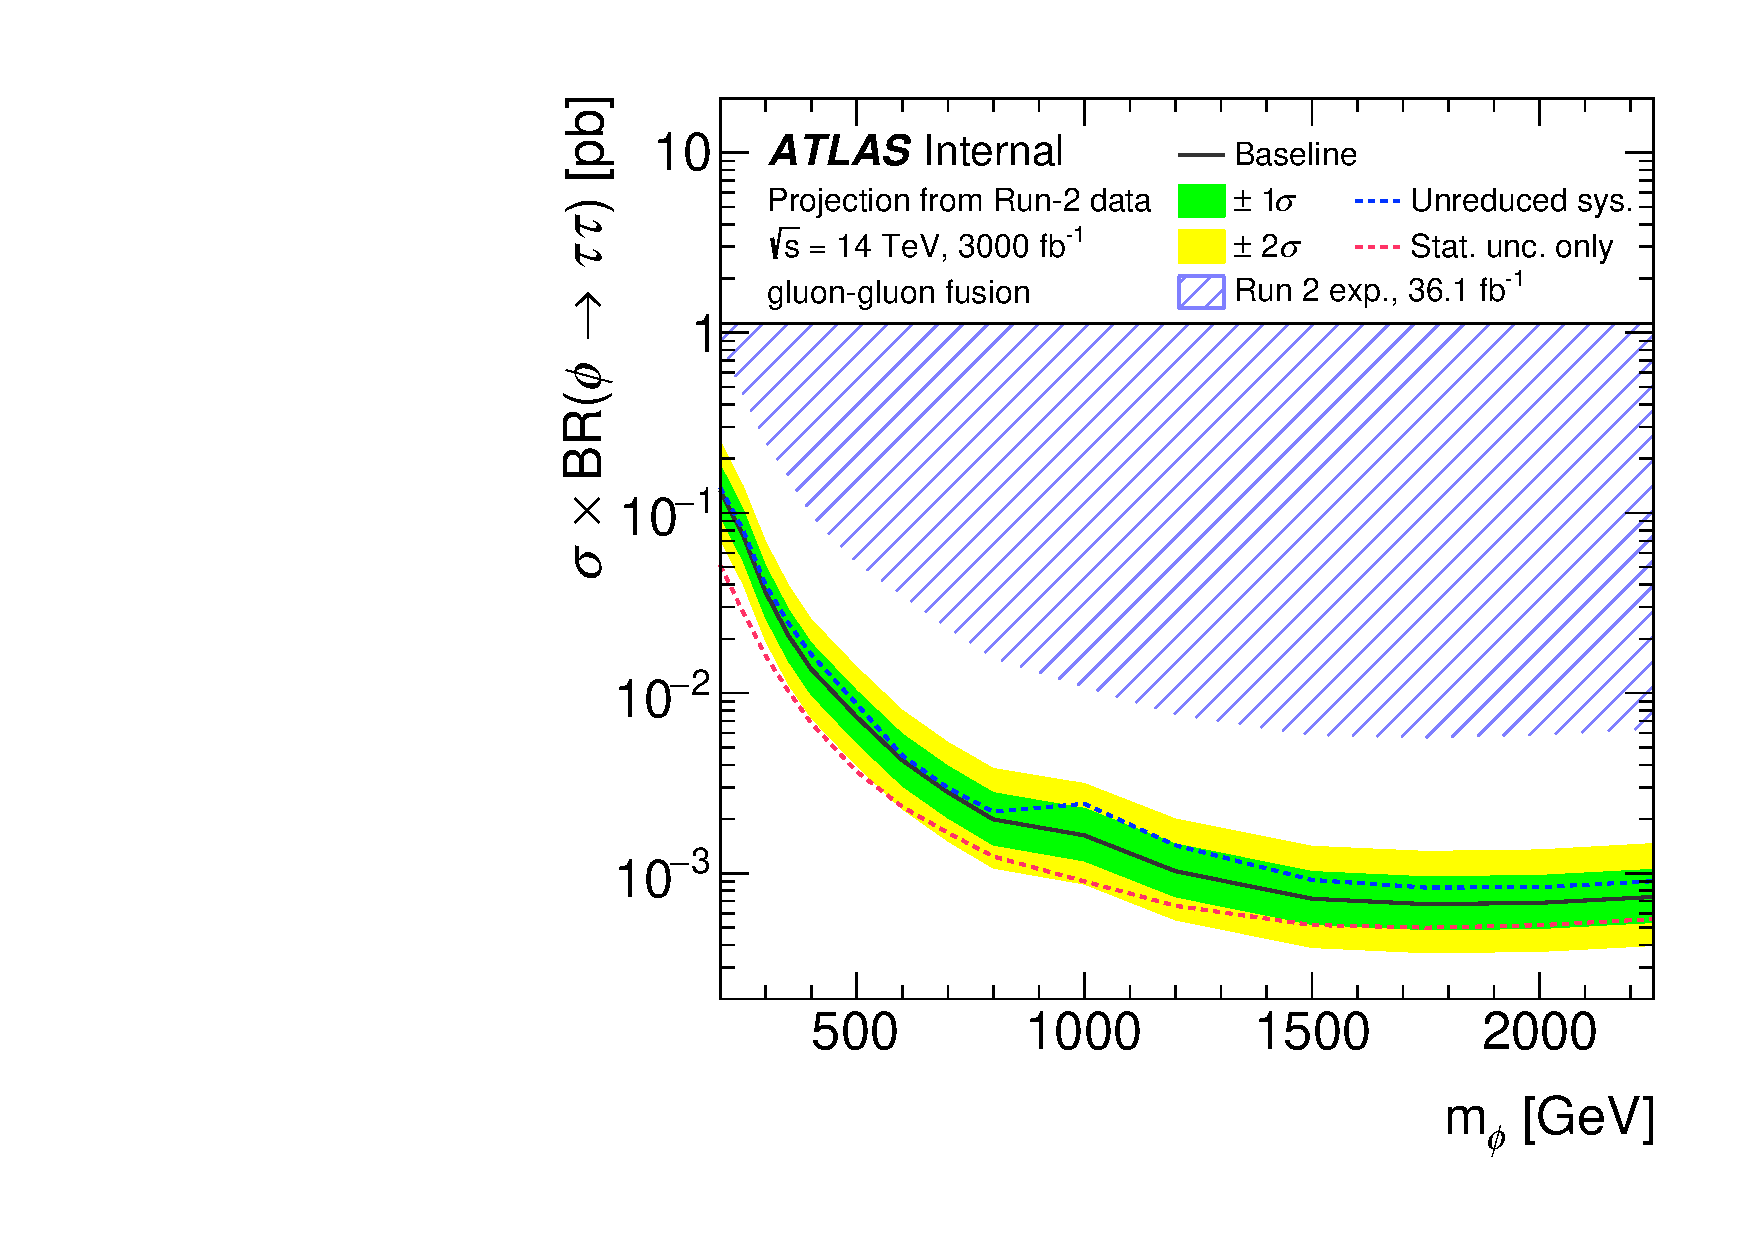
\includegraphics[width=0.4\columnwidth]{\main/section9/plots/ggH.pdf}}
        \qquad
        \subfloat[$b$-associated production\label{fig:modelInde, bbH}]{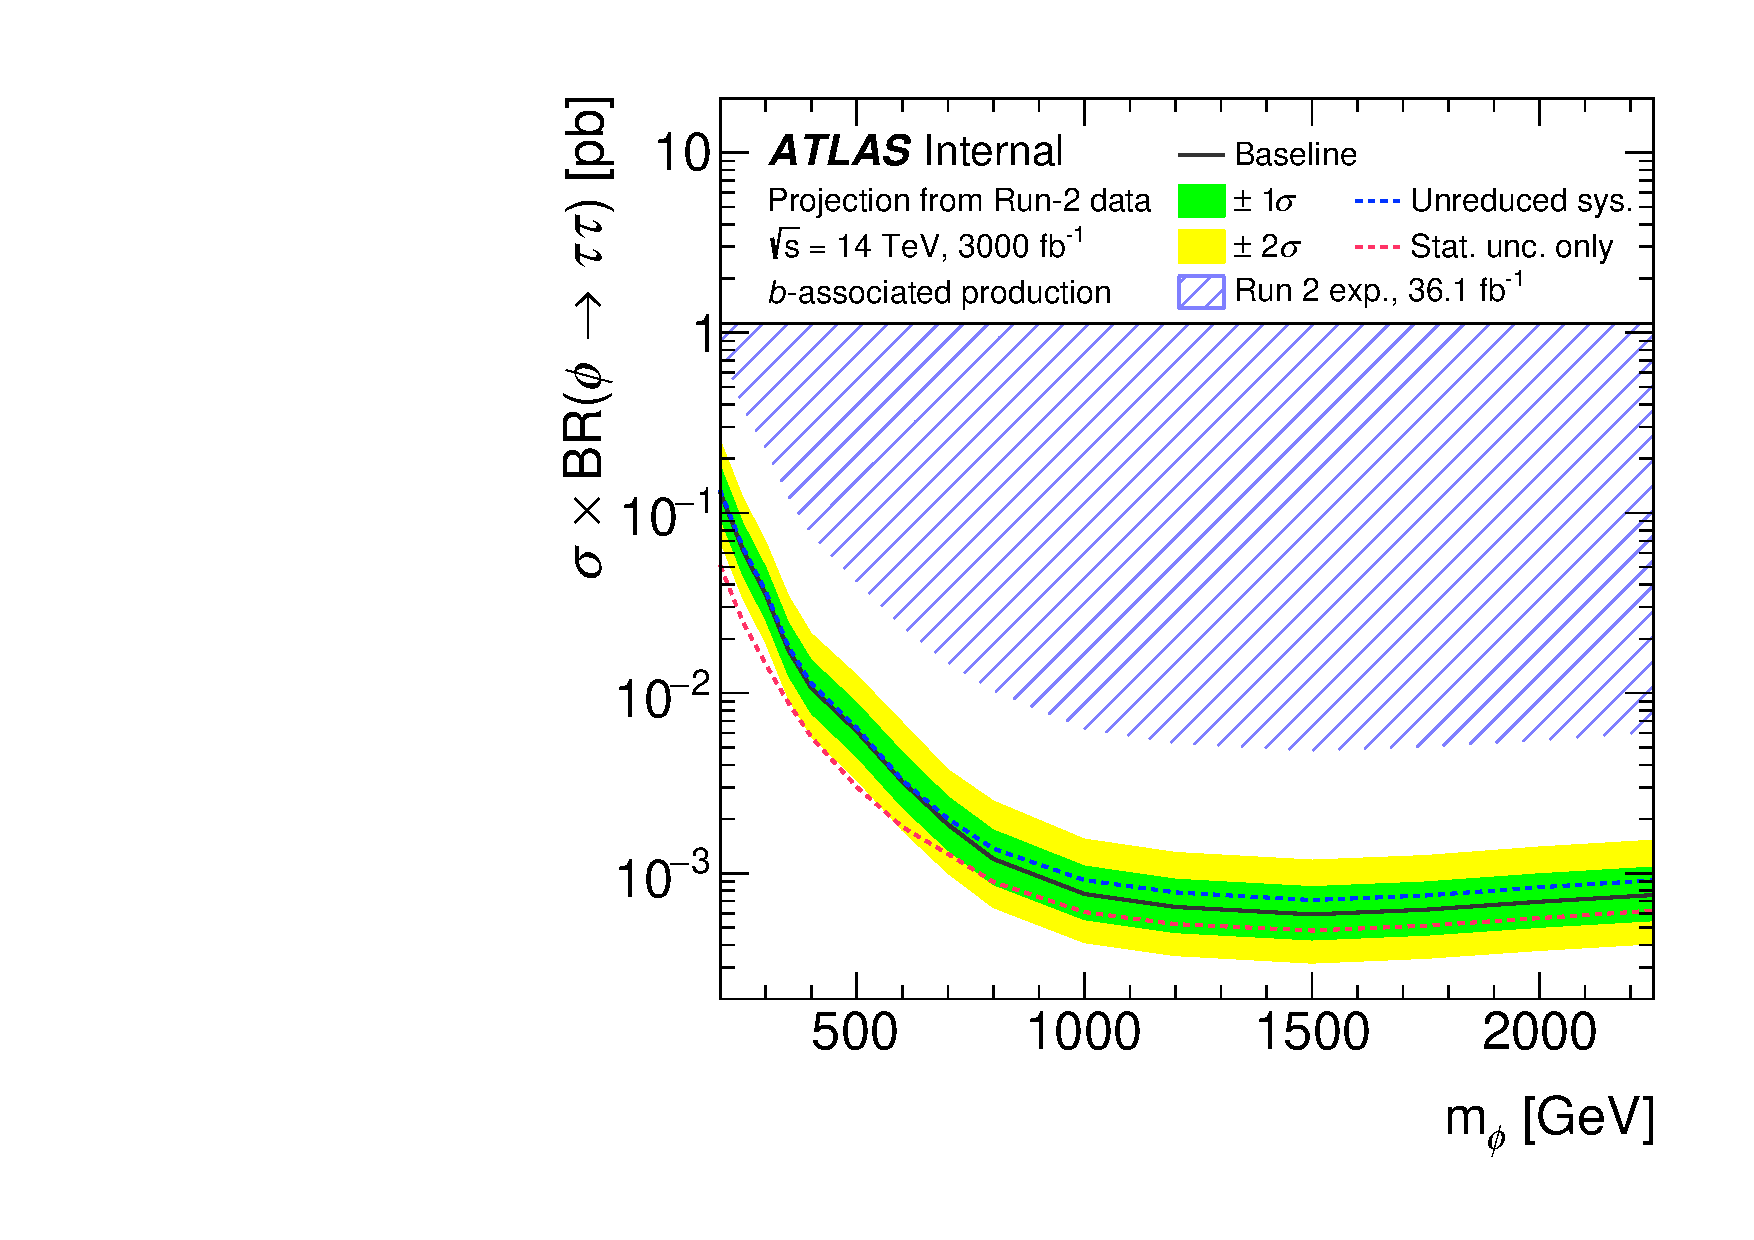
\includegraphics[width=0.4\columnwidth]{\main/section9/plots/bbH.pdf}}
        \caption{
         Projected 95\% CL upper limits on the production cross section times the $\phi\rightarrow\tau\tau$ branching fraction for a scalar boson $\phi$ produced via (a) gluon--gluon fusion and (b) $b$-associated production, as a function of scalar boson mass. The limits are calculated from a statistical combination of the \ehad, \muhad and \hadhad channels. ``Baseline'' uses the reduced systematic uncertainties scenario described in the text. ``Unreduced sys.\@'' uses the same systematic uncertainties as the Run 2 analysis while ignoring the template stat.\@ uncertainty. ``Stat.\@ unc.\@ only'' represents the expected limit without considering any systematic uncertainty. ``5 $\sigma$ sensitivity'' shows the region with the potential of 5 $\sigma$ significance in the Baseline scenario.
        }
    \label{fig:modelInde}
\end{figure}

\begin{figure}[!ht]
    \centering
        \subfloat[gluon--gluon fusion production]{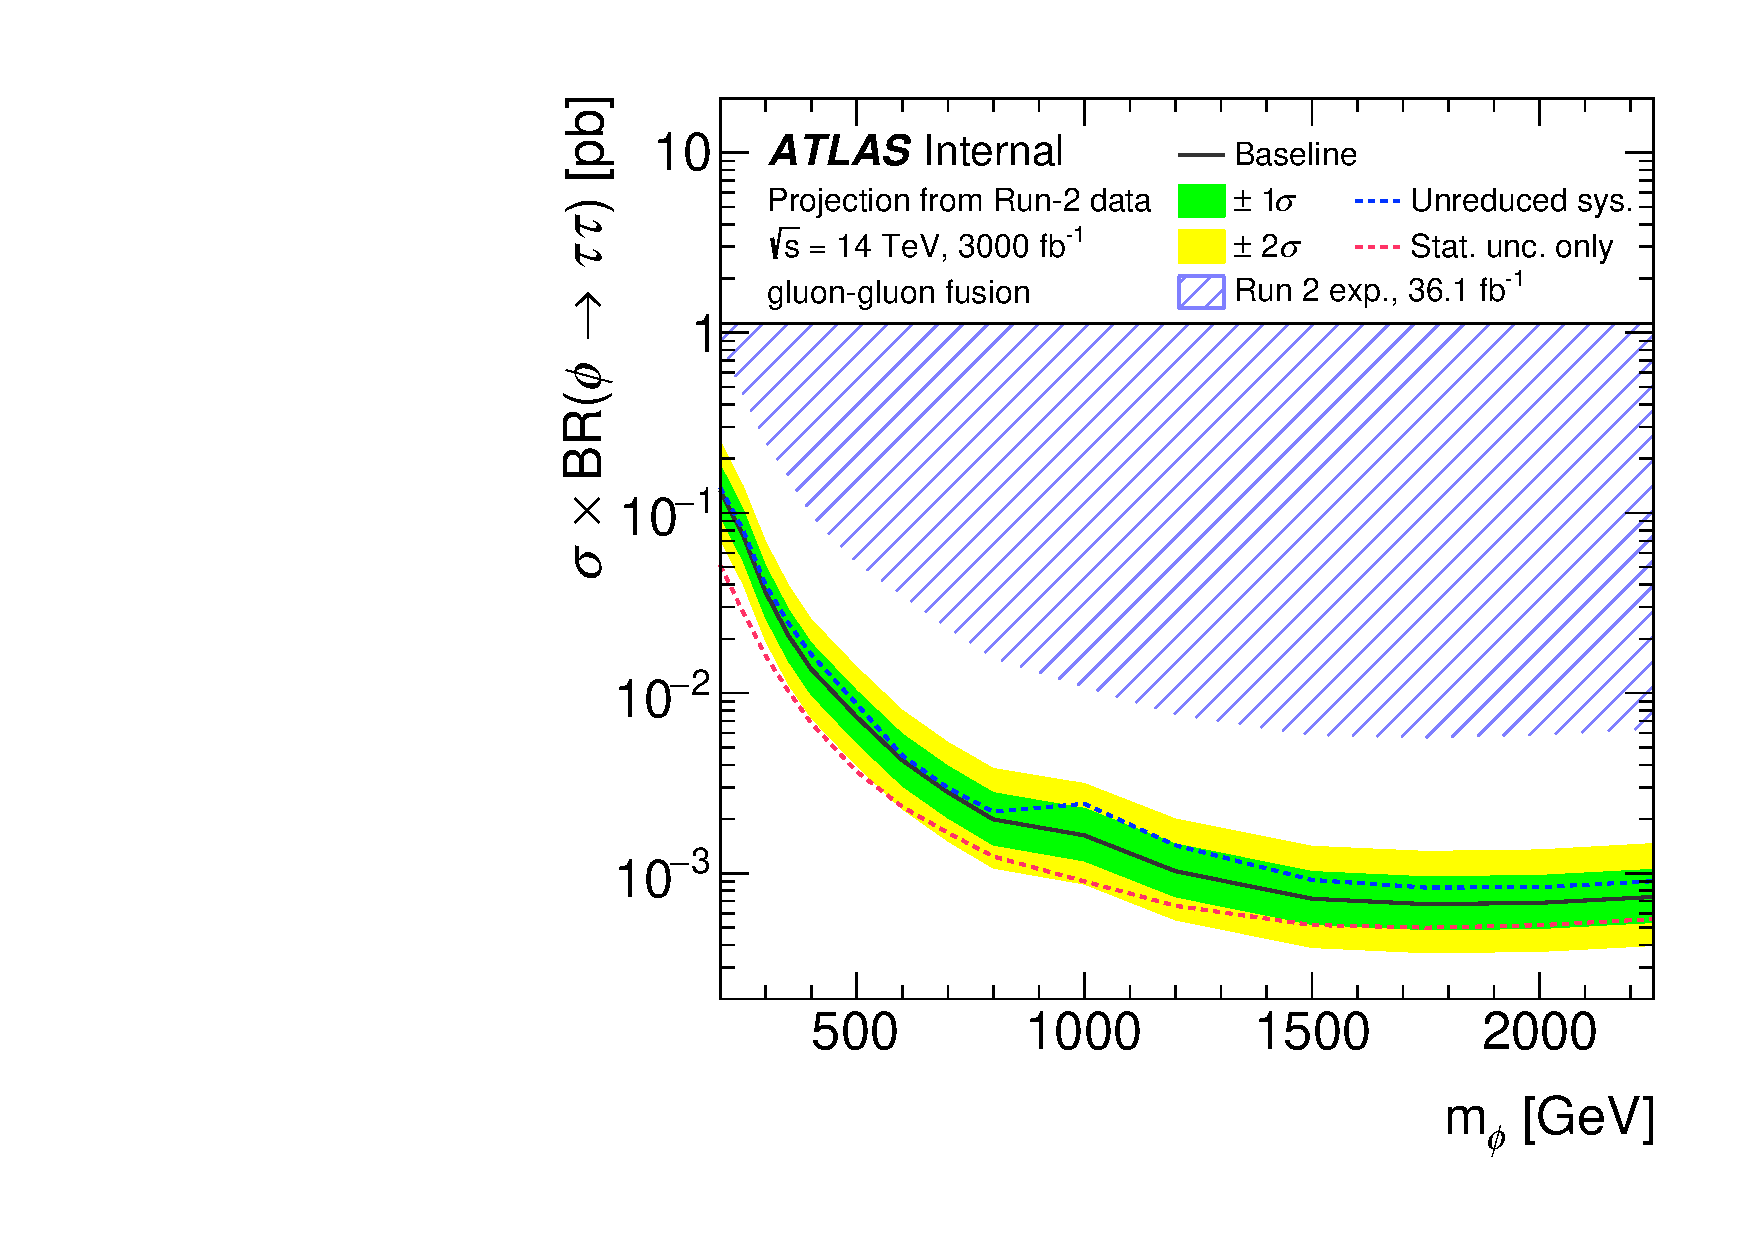
\includegraphics[width=0.4\columnwidth]{\main/section9/plots/ggH.pdf}}
        \qquad
        \subfloat[$b$-associated production]{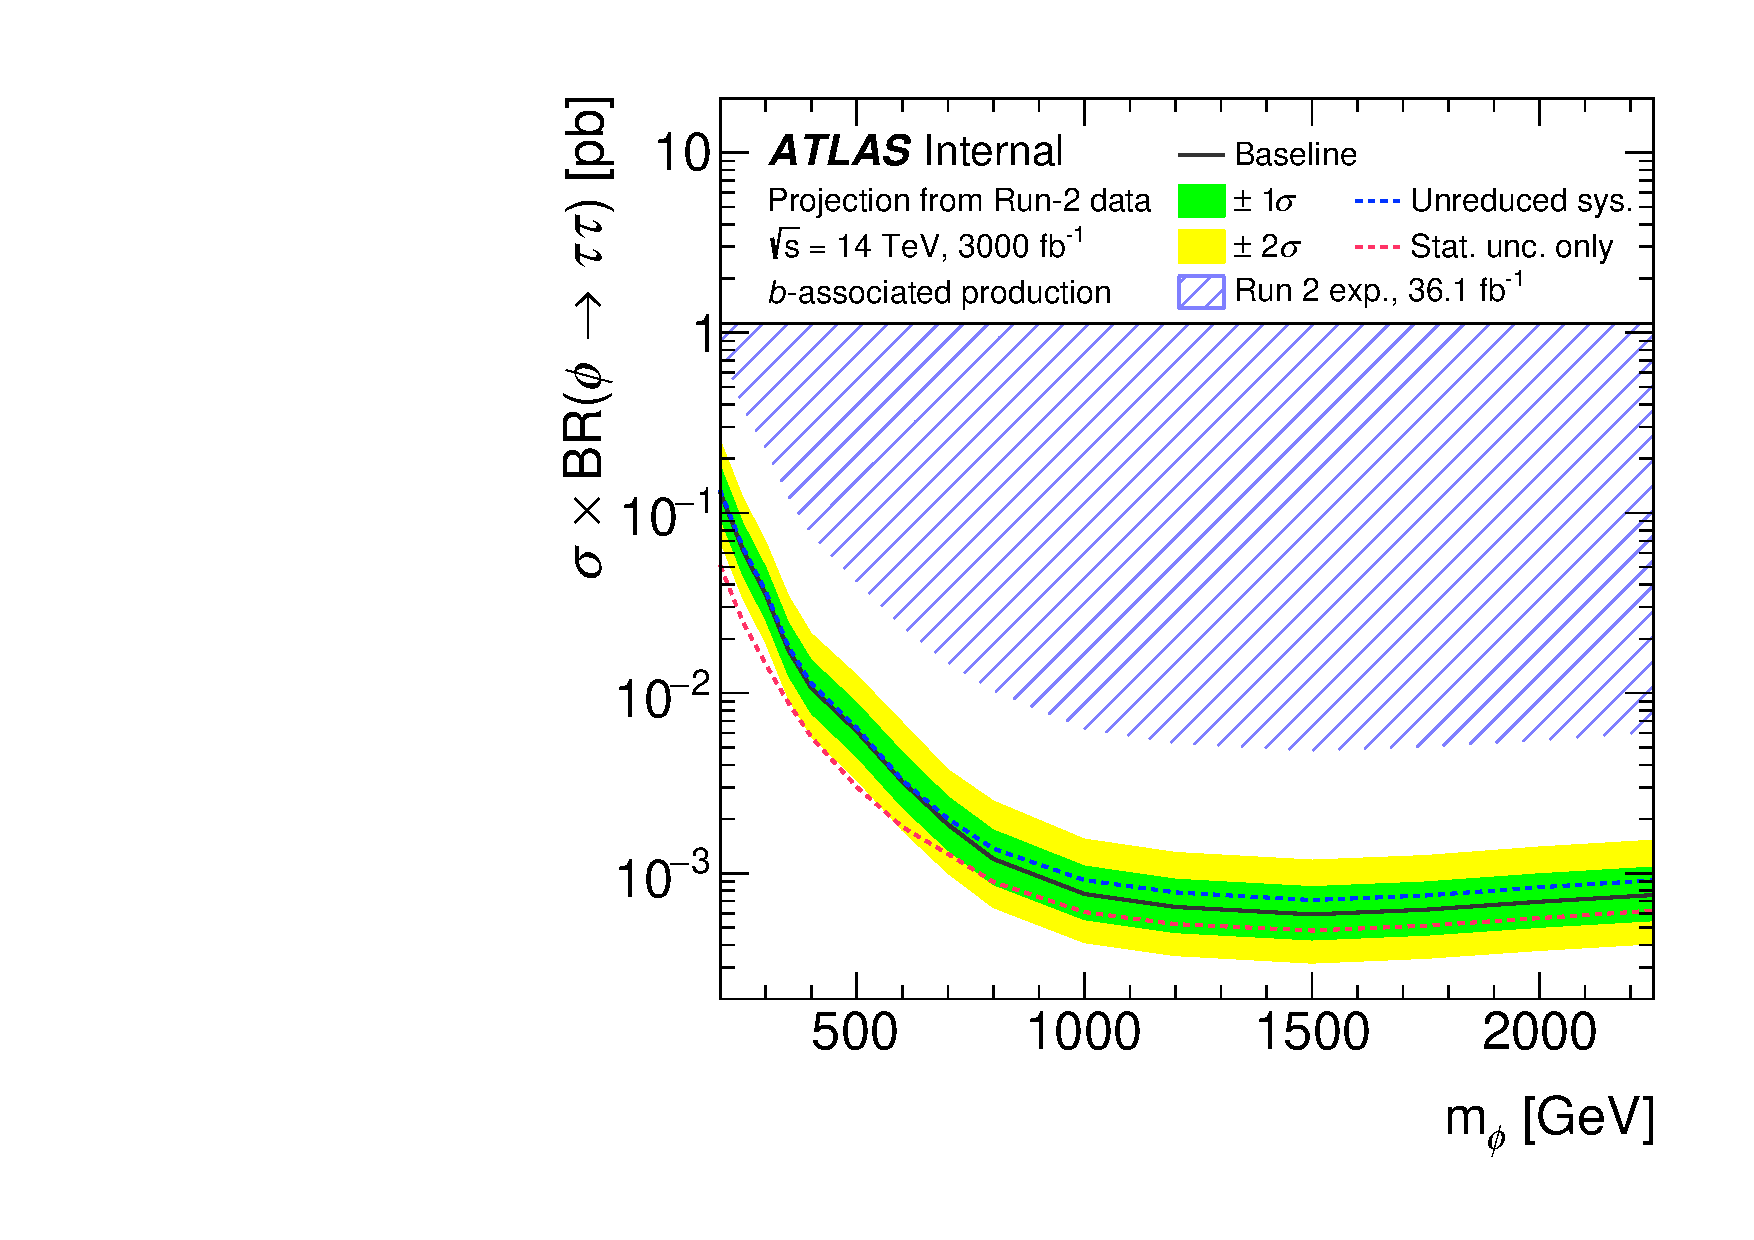
\includegraphics[width=0.4\columnwidth]{\main/section9/plots/bbH.pdf}}
        \caption{Projected 95\% CL upper limits on the production cross section times ditau branching fraction for a scalar boson produced via (a) gluon--gluon fusion and (b) $b$-associated production, as a function of scalar boson mass. The limits are calculated from a statistical combination of the \ehad, \muhad and \hadhad channels. ``Baseline'' uses the reduced systematic uncertainties scheme described in the text. ``Unreduced sys.'' uses the same systematic uncertainties as the Run 2 analysis while ignoring the statistical uncertainty due to the limited data size of the signal and backgrounds. ``Stat. unc. only'' represents the expected limit without considering any systematic uncertainty.
        }
    \label{fig:modelInde}
\end{figure}

\paragraph{MSSM interpretation}
Results are interpreted in terms of the MSSM\@. The cross section calculations follow the exact procedure used in Ref.~\cite{ATLASRun2Ditau}, apart from the centre of mass energy is switched to 14~\TeV. Figure~\ref{fig:model1} shows regions in the $m_A$--$\tan\beta$ plane excluded at 95\% CL or discovered with 5 $\sigma$ significance in the hMSSM and \mhmodp scenarios. In the hMSSM scenario, $\tan\beta > 1.0$ for $250< m_A < 350$~\GeV and $\tan\beta > 10$ for $m_A = 1.5~\TeV$ could be excluded at 95\% CL\@. When $m_A$ is above the $A/H\to \ttbar$ threshold, this additional decay mode reduces the sensitivity of the $A/H\to\tau\tau$ search for low $\tan\beta$. In the MSSM \mhmodp scenario, the expected 95\% CL upper limits exclude $\tan\beta >2$ for $250< m_A< 350$~\GeV and $\tan\beta > 20$ for $m_A =1.5~\TeV$.

\begin{figure}[!ht]
    \centering
        \subfloat[hMSSM scenario]{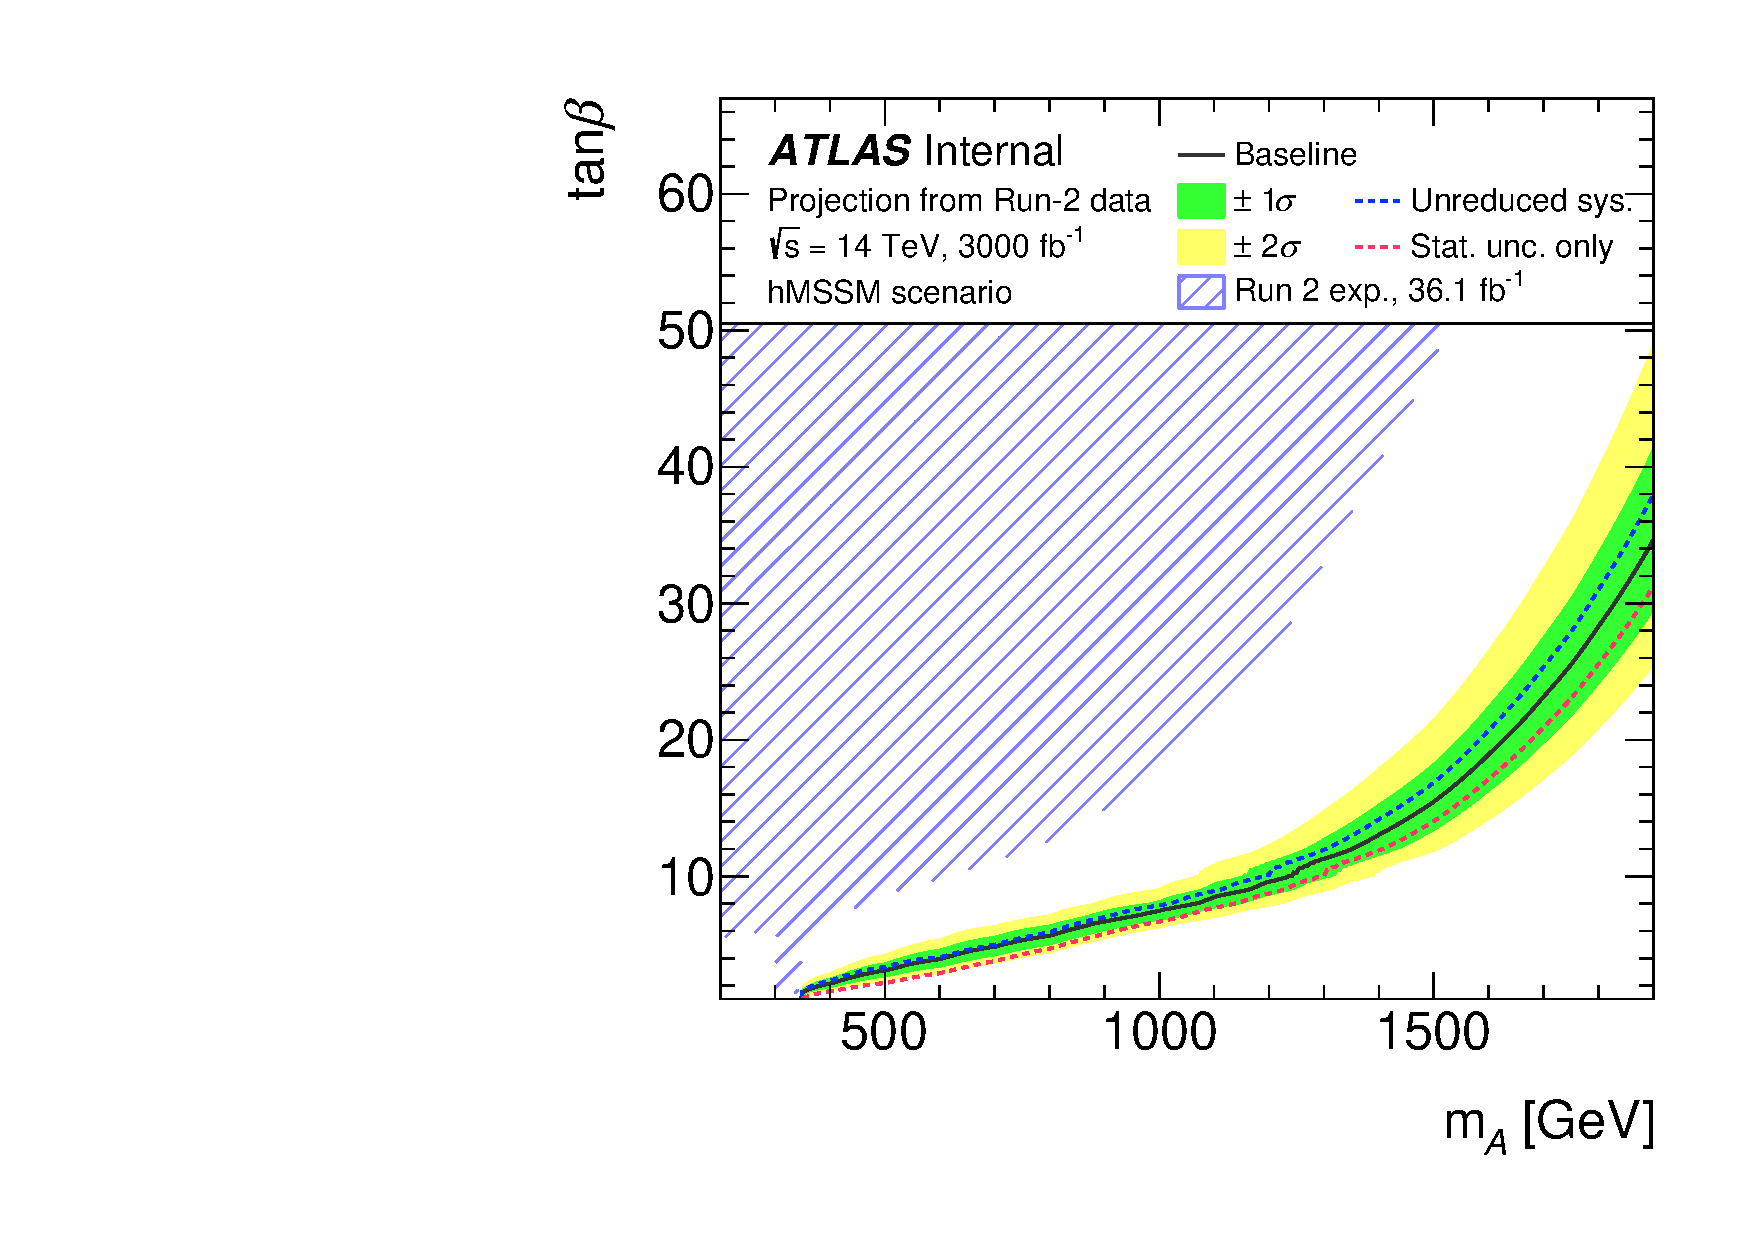
\includegraphics[width=0.4\columnwidth]{\main/section9/plots/hMSSM.pdf}}
        \qquad
        \subfloat[\mhmodp scenario]{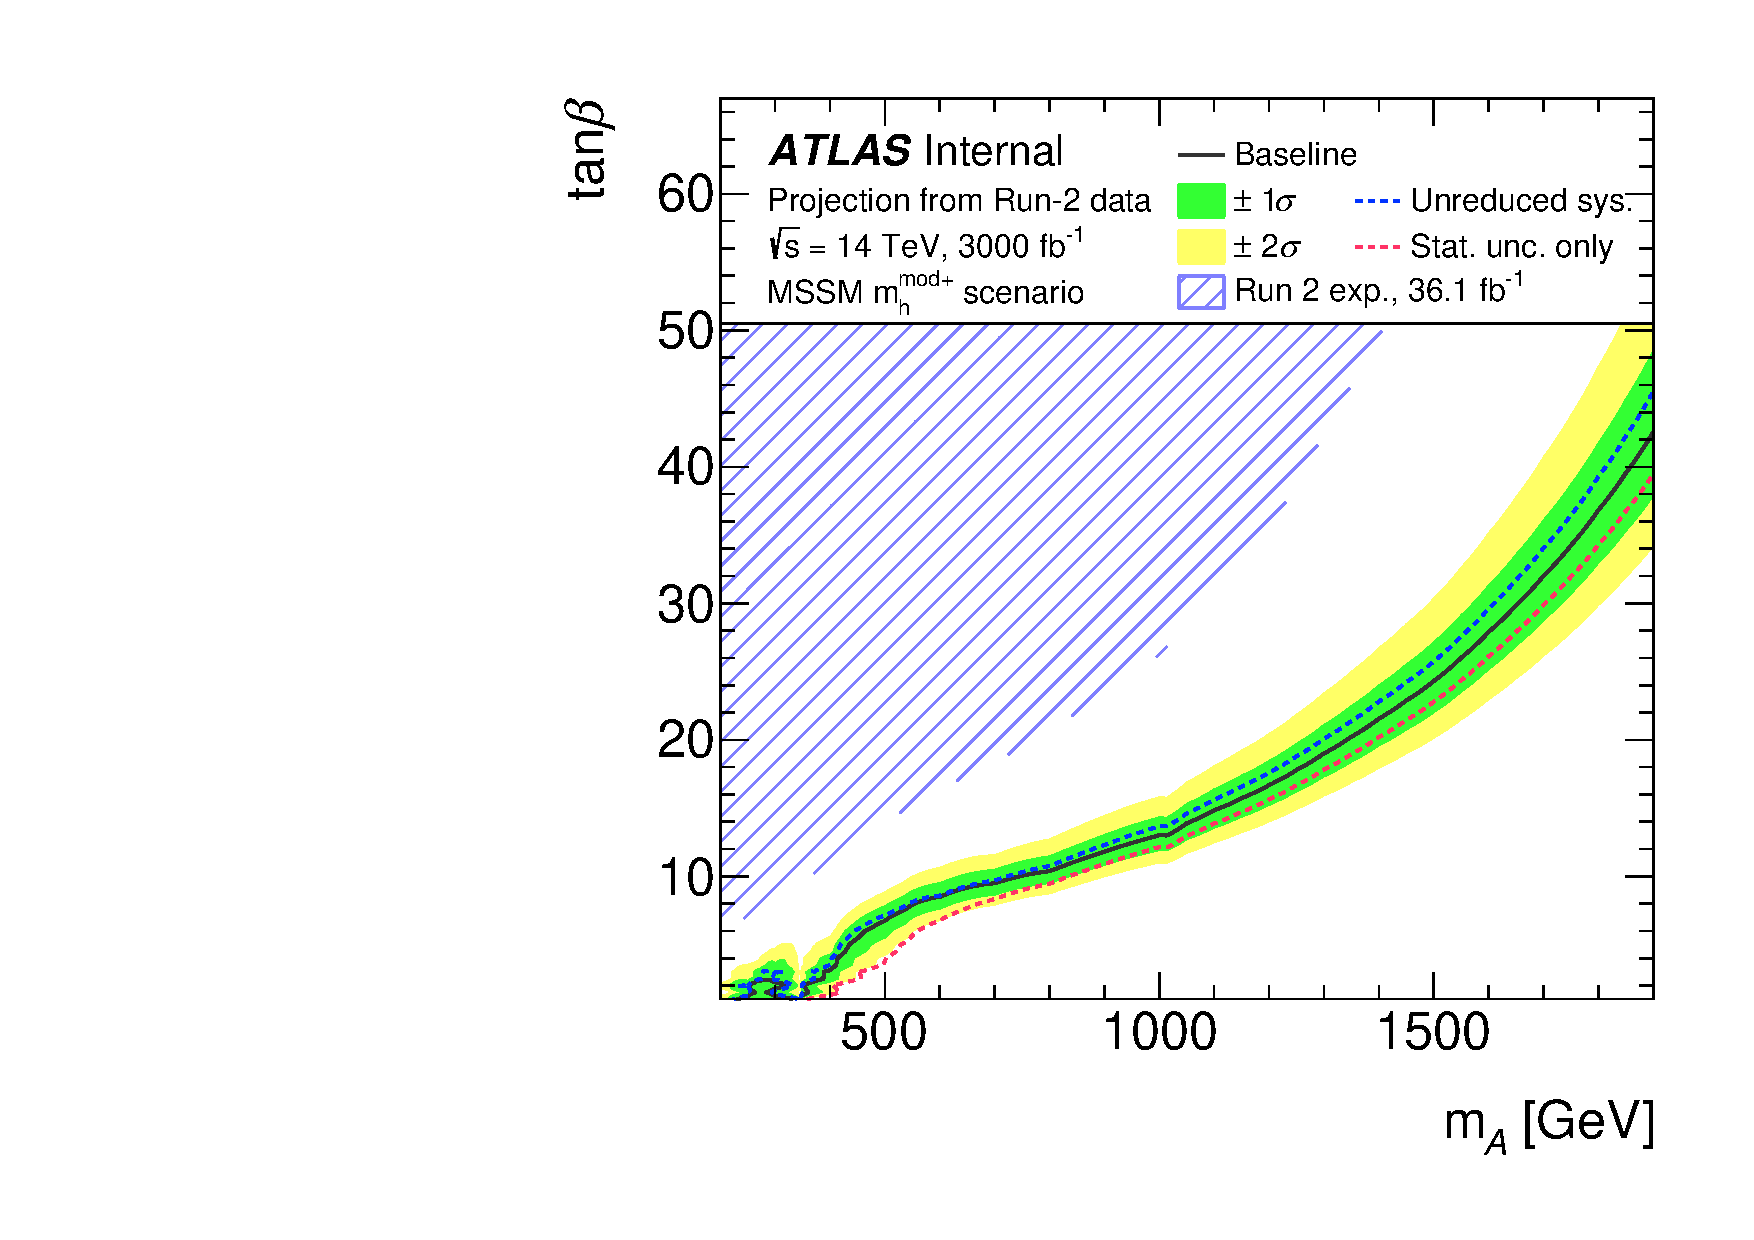
\includegraphics[width=0.4\columnwidth]{\main/section9/plots/mhmodp.pdf}}
        \caption{Projected 95\% CL limits on $\tan\beta$ as a function of $m_\phi$ in the MSSM (a) hMSSM and (b) \mhmodp scenarios. The limits are calculated from a statistical combination of the \ehad, \muhad and \hadhad channels. ``Baseline'' uses the reduced systematic uncertainties scenario described in the text. ``Unreduced sys.\@'' uses the same systematic uncertainties as the Run 2 analysis while ignoring the template stat.\@ uncertainty. ``Stat.\@ unc.\@ only'' represents the expected limit without considering any systematic uncertainty. ``5 $\sigma$ sensitivity'' shows the region with the potential of 5 $\sigma$ significance in the Baseline scenario.
        }
    \label{fig:model1}
\end{figure}

\FloatBarrier

%-------------------------------------------------------------------------------
\paragraph{Conclusion}
\label{sec:conclusion}
%-------------------------------------------------------------------------------
The $H/A \to \tau\tau$ analysis documented in \cite{ATLASRun2Ditau} has been extrapolated to estimate the sensitivity with $3000~\ifb$ of the HL-LHC dataset. The expected upper limits at 95\% CL or, in alternative, the 5 $\sigma$ discovery reach in terms of cross section for the production of scalar bosons times the branching fraction to ditau final states have been estimated. The region with 5 $\sigma$ discovery potential at HL-LHC extends significantly below the currently expected Run 2 exclusion region. The expected limits are in the range 130--0.4~$\fb$ (130--0.3~$\fb$) for gluon--gluon fusion ($b$-associated) production of scalar bosons with masses of 0.2--2.25~$\TeV$. A factor of 6 to 18 increase in the sensitivity compared to the searches with the 36.1~$\ifb$ Run 2 data~\cite{ATLASRun2Ditau} is projected. In the context of the hMSSM scenario, in the absence of a signal, the most stringent limits expected for the combined search exclude $\tan\beta > 1.0$ for $250 < m_A < 350$ \si{\GeV} and $\tan\beta > 10$ for $m_A = 1.5~\TeV$ at 95\% CL\@. The systematic uncertainties degrade the exclusion limit on $\sigma\times BR(\phi\to\tau\tau)$ by more than a factor of 2 for $m_\phi<500~\GeV$ and about 10\%--20\% for $m_\phi= 2~\TeV$. While the uncertainty on the estimate of fake $\tauhad$ dominates at low $m_{\phi}$, the uncertainty on high-$\pt$ $\tauhad$ reconstruction and identification is the leading systematic uncertainty at $m_\phi > 1.0~\TeV$.